
\section{McSat: An extension of SMT Solvers}

\subsection{Introduction}

Introduced in~\cite{VMCAI13} and~\cite{FMCAD13}.

Mcsat is an extension of usual SMT solvers. In usual SMT Solvers, interaction between
the core SAT Solver and the Theory is pretty limited~: the SAT Solver sends the boolean
assignments it makes to the theory, which then can eventually stop the SAT Solver by
saying the current set of assumptions, viewed as a conjunction, is incoherent. This means
that if we exclude the backtracking phase of the SMT Solver, information only goes one way:
from the SAT Solver to the theory.

While it is sound and complete, in some cases, it might be useful to allow information to
travel in the two directions: for instance, if the SAT Solver assumes $x = 0$, the theory
could tell the SAT Solver that the formula $x < 1$ must also hold, instead of waiting
for the SAT Solver to guess its truth value, and then inform the SAT Solver that the
conjunction~: $x = 0 \land \neg x < 1$ is incoherent. To that effect, in McSat,
the SAT Solver not only decides on boolean assignments for the literals in its clauses,
but only on assignments of terms inside those formulas.

\subsection{SMT Solver architecture}

We can represent a simplified version of the control flow of SMT Solvers by the
graph in fig~\ref{fig:smt_flow}. In a pure Sat solver, the solver starts by doing
boolean propagation until no more literal can be propagated, at which point it
makes a decision and assign a truth value to a literal not yet assigned. It then
loops to its starting point and does boolean propagation. In an Smt solver,
after each boolean propagation, the solver sends the newly assigned literals
to the theory. The only way for the theory to give back information is to
declare the current set of literals incoherent, and give the solver a tautology
which evaluates to $\bot$ in the current assignment.

\begin{figure}
  \begin{center}
    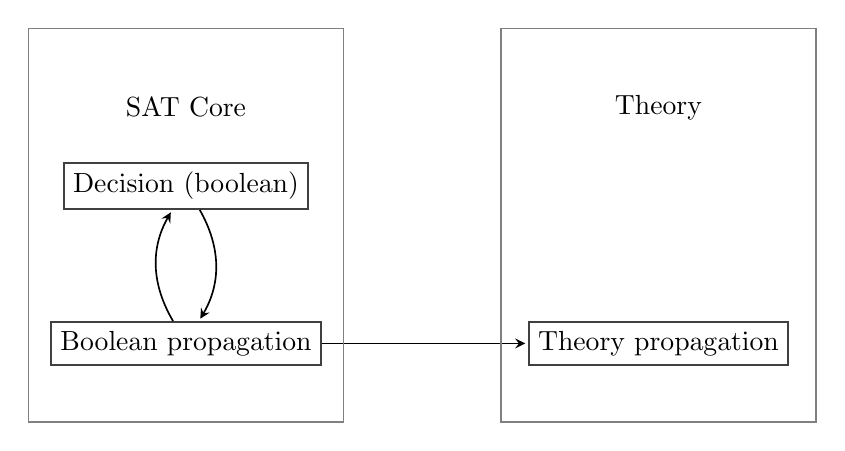
\begin{tikzpicture}[
        ->, % Arrow style
        > = stealth, % arrow head style
        shorten > = 1pt, % don't touch arrow head to node
        node distance = 2cm, % distance between nodes
        semithick, % line style
        auto
      ]

      \tikzstyle{state}=[rectangle,draw=black!75]

      \node (sat) {SAT Core};
      \node (th) [right of=sat, node distance=6cm] {Theory};
      \node[state] (d) [below of=sat, node distance=1cm] {Decision (boolean)};
      \node[state] (bp) [below of=d, node distance=2cm] {Boolean propagation};
      \node[state] (tp) [right of=bp, node distance=6cm] {Theory propagation};

      \path (d) edge [bend left=30] (bp);
      \path (bp) edge [bend left=30] (d);
      \path (bp) edge (tp);

      \draw[black!50] (-2,1) rectangle (2,-4);
      \draw[black!50] (4,1) rectangle (8,-4);

    \end{tikzpicture}
  \end{center}
  \caption{Simplified SMT Solver architecture}\label{fig:smt_flow}
\end{figure}

The main addition of McSat is that when the solver makes a decision, instead of
being restricted to making boolean assignment of formulas, the solver now can
decide to assign a term belonging to one of the literals. In order to do so,
the solver asks the theory for a possible assignment. Since terms can have
assignments, the theory can now do useful and efficient propagation on its
side, and propagate the truth value of formulas for which all the terms
have been assigned. The modified control flow then looks like
fig~\ref{fig:mcsat_flow}.

For a more detailed presentation, see~\cite{FMCAD13} and~\cite{VMCAI13}.

\begin{figure}
  \begin{center}
    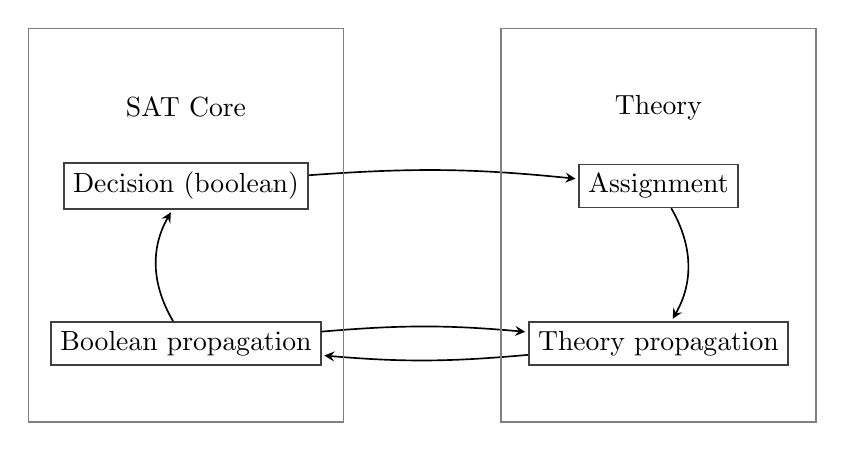
\begin{tikzpicture}[
        ->, % Arrow style
        > = stealth, % arrow head style
        shorten > = 1pt, % don't touch arrow head to node
        node distance = 2cm, % distance between nodes
        semithick, % line style
        auto
      ]

      \tikzstyle{state}=[rectangle,draw=black!75]

      \node (sat) {SAT Core};
      \node (th) [right of=sat, node distance=6cm] {Theory};
      \node[state] (d) [below of=sat, node distance=1cm] {Decision (boolean)};
      \node[state] (ass) [right of=d, node distance=6cm] {Assignment};
      \node[state] (bp) [below of=d, node distance=2cm] {Boolean propagation};
      \node[state] (tp) [right of=bp, node distance=6cm] {Theory propagation};

      \path (bp)[right] edge [bend left=5] (tp);
      \path (tp) edge [bend left=5] (bp);
      \path (bp) edge [bend left=30] (d);
      \path (d) edge [bend left=5] (ass);
      \path (ass) edge [bend left=30] (tp);

      \draw[black!50] (-2,1) rectangle (2,-4);
      \draw[black!50] (4,1) rectangle (8,-4);

    \end{tikzpicture}
  \end{center}
  \caption{Simplified McSat Solver architecture}\label{fig:mcsat_flow}
\end{figure}

\subsection{Expected theory invariants}

In exchange for the responsibility of producing possible assignments,
the theory now bears a little less responsibility, more specifically,
it has to enforce different invariants than in a traditional SMT Solver.

Usually, the main invariant enforced by the theory is the coherence of
the conjunction of all formulas asserted by the solve so far.
In a McSat solver, the theory is allowed to maintain a weaker invariant,
which is that it must be able to produce an assignment for any term
that belongs to the problem. In other words, given any state of the solver
with a current assignment $\sigma$ and a set of assertions $S$ (i.e all
formulas in $S$ have been assigned to $\top$ by the solver\footnote{In case it is
unclear, assigning a formula $f$ to $\bot$ is equivalent to assigning  $\neg f$ to $\top$}),
for each term $t$, the theory must be able to produce a value $v$
such that $\bigwedge_{f \in S} f\sigma'$ is not incoherent, with
$\sigma' = \sigma \cup \{ t \rightarrow v \}$. Note that this does not
mean that $\bigwedge_{f\in S} f\sigma'$ is satisfiable. Rather, it means that
the theory is capable of producing an assignment that does not directly
contradicts the current boolean assignment.


